\chapter{Evaluation and Analysis}

In the previous chapter, a few approaches that could improve the genetic solver were presented.
The best results give a combination of the genetic solver with added probabilities and parameter tuning.
Other methods like an adaptive crossover rate or population without duplicated individuals give less effect on the results.

On the other hand, we get valid results only for one problem. What if the problem will be smaller or bigger?
The evaluation was done to find out how all approaches work with different problem sizes. 

\section{Evaluation}

To evaluate genetic solver, a benchmark set of 36 problems was used.
Each problem with different parameters that describes them.
All parameters are:

\begin{itemize}
	\item variant - [2, 4] ,
	\item request - [1, 2, 4],
	\item depth - [2, 3, 4],
	\item resources - [50, 100].
\end{itemize}

This set was tested with several versions of the genetic solver:

\begin{itemize}
	\item basic (B),
	\item basic with tuned parameters (B-T),
	\item without hard-coded parameters and tuning (WHC-T) 
	\item with added parameters (NP),
	\item with added parameters and tuning (NP-T),
	\item with internally changeable crossover rate (ICCR),
	\item with internally changeable crossover rate and tuning (ICCR-T),
	\item without duplicates in the population (WD),
	\item without duplicates in the population and tuning (WD-T).
\end{itemize}

Each version of the genetic solver tries five times to solve each problem.

The benchmark set was run on an Intel Core i7-8700 CPU machine with 64Gb of memory using Fedora Server 29 and OpenJDK 1.8.0 201-b09.

Benchmark trying so solve each task, if a solution was valid, genetic solver start to solve next problem. If after five attempts the genetic solver did not find a valid solution, it proceeded to the next problem.

\begin{figure}
	\centering
	\includegraphics[width=\textwidth]{images/EvaluationNumberOfSolvedProblems.pdf}
	\caption[Number of problems for each version of the genetic solver]{Number of solved problems for each version of the genetic solver}
	\label{fig:EvaluationNumberOfSolvedProblems}
\end{figure}

Figure~\ref{fig:EvaluationNumberOfSolvedProblems} results of the benchmark. For each version of the genetic solver, a vertical bar was built. The height of the bar shows the number of solved problems from the benchmark set. The B version solved the least of problems than any other version. Almost in all cases, parameter tuning increases the number of solved problems. It also confirms the answer to \textbf{RQ1}. The comparison of N-T, WHC-T, and NP versions shows that the NP bar is higher than N-T but lower than WHC-T. This comparison confirms the first conclusion from Section~\ref{sec:NP}, that well-designed parameters are important for any algorithm. The combination of parameter engineering and parameter tuning in NP-T gives the best results. The same situation was for one problem in the previous chapter~(Figure~\ref{fig:boxplotsolverNoDuplicates}). The WD-T gives worse results than the untuned version. The possible reasons for such results were discussed in Section~\ref{sec:WD}. The result of the benchmark for the ICCR-T version contradicts the results obtained in the last section because the parameter tuning of the ICCR version gives the biggest improvement. In general, benchmark results for a set of 36 MQuAT problems correspond to the results for one problem.

The benchmark also shows that no one version of the genetic solver solved all problems from the set.

\begin{table}
	\centering
	\caption{Problem color coding}\label{tab:ProblemsColorCoding}
	\resizebox*{\textwidth}{\textheight}{
		\begin{tabular}{c c c c c c c c c c}
			\hline
			\rotatebox{90}{Problem Id} & \rotatebox{90}{B} & \rotatebox{90}{B-T} & \rotatebox{90}{WHC-T} & \rotatebox{90}{NP} & \rotatebox{90}{NP-T} & \rotatebox{90}{ICCR} & \rotatebox{90}{ICCR-T} & \rotatebox{90}{WD} & \rotatebox{90}{WD-T} \\
			\hline			
			1 & \cellcolor{lightgray} & \cellcolor{Gray} & \cellcolor{black} & \cellcolor{yellow} & \cellcolor{orange} & \cellcolor{red} & \cellcolor{brown} & \cellcolor{lime} & \cellcolor{green} \\ 
			2 &   &   & \cellcolor{black} &   & \cellcolor{orange} &   &   & \cellcolor{lime} & \cellcolor{green}  \\
			3 &   &   &   &   & \cellcolor{orange} &   &   & \cellcolor{lime} &  \\
			4 &   & \cellcolor{Gray} & \cellcolor{black} & \cellcolor{yellow} & \cellcolor{orange} & \cellcolor{red} & \cellcolor{brown} & \cellcolor{lime} & \cellcolor{green} \\
			5 &   &   &   &   & \cellcolor{orange} &   & \cellcolor{brown} &   & \\
			6 &   &   &   &   &   &   &   &   & \\
			7 &   & \cellcolor{Gray} & \cellcolor{black} & \cellcolor{yellow} & \cellcolor{orange} &   & \cellcolor{brown} & \cellcolor{lime} & \cellcolor{green}\\
			8 &   &   &   &   &   &   &   &   & \\
			9 &   &   &   &   &   &   &   &   & \\
			10 & \cellcolor{lightgray} & \cellcolor{Gray} & \cellcolor{black} & \cellcolor{yellow} & \cellcolor{orange} & \cellcolor{red} & \cellcolor{brown} & \cellcolor{lime} & \cellcolor{green} \\
			11 &   &   & \cellcolor{black} & \cellcolor{yellow} & \cellcolor{orange} & \cellcolor{red} & \cellcolor{brown} & \cellcolor{lime} & \cellcolor{green} \\
			12 &   &   &   &   & \cellcolor{orange} &   & \cellcolor{brown} & \cellcolor{lime} &   \\
			13 & \cellcolor{lightgray} & \cellcolor{Gray} & \cellcolor{black} & \cellcolor{yellow} & \cellcolor{orange} & \cellcolor{red} & \cellcolor{brown} & \cellcolor{lime} & \cellcolor{green} \\
			14 &   &   &   &   & \cellcolor{orange} &   & \cellcolor{brown} &   &   \\
			15 &   &   &   &   &   &   &   &   & \\
			16 &   & \cellcolor{Gray} & \cellcolor{black} & \cellcolor{yellow} & \cellcolor{orange} &   & \cellcolor{brown} &   & \cellcolor{green} \\
			17 &   &   &   &   &   &   &   &   & \\
			18 &   &   &   &   &   &   &   &   & \\
			19 & \cellcolor{lightgray} & \cellcolor{Gray} & \cellcolor{black} & \cellcolor{yellow} & \cellcolor{orange} & \cellcolor{red} & \cellcolor{brown} & \cellcolor{lime} & \cellcolor{green}\\
			20 &   &   & \cellcolor{black} & \cellcolor{yellow} & \cellcolor{orange} & \cellcolor{red} & \cellcolor{brown} & \cellcolor{lime} & \cellcolor{green} \\
			21 &   &   &   &   & \cellcolor{orange} &   & \cellcolor{brown} &   & \\
			22 & \cellcolor{lightgray} & \cellcolor{Gray} & \cellcolor{black} &   & \cellcolor{orange} & \cellcolor{red} & \cellcolor{brown} & \cellcolor{lime} & \cellcolor{green} \\
			23 &   &   & \cellcolor{black} & \cellcolor{yellow} & \cellcolor{orange} &   & \cellcolor{brown} & \cellcolor{lime} &  \\
			24 &   &   &   &   &   &   &   &   & \\
			25 &   &   & \cellcolor{black} & \cellcolor{yellow} & \cellcolor{orange} &   & \cellcolor{brown} &   & \cellcolor{green} \\
			26 &   &   &   &   &   &   &   &   & \\
			27 &   &   &   &   &   &   &   &   & \\
			28 & \cellcolor{lightgray} & \cellcolor{Gray} & \cellcolor{black} & \cellcolor{yellow} & \cellcolor{orange} & \cellcolor{red} & \cellcolor{brown} & \cellcolor{lime} & \cellcolor{green} \\
			29 &   & \cellcolor{Gray} & \cellcolor{black} & \cellcolor{yellow} & \cellcolor{orange} & \cellcolor{red} & \cellcolor{brown} & \cellcolor{lime} & \cellcolor{green} \\
			30 &   &   &   &   &   &   &   &   & \\
			31 & \cellcolor{lightgray} & \cellcolor{Gray} & \cellcolor{black} & \cellcolor{yellow} & \cellcolor{orange} & \cellcolor{red} & \cellcolor{brown} & \cellcolor{lime} & \cellcolor{green} \\
			32 &   &   & \cellcolor{black} & \cellcolor{yellow} & \cellcolor{orange} &   & \cellcolor{brown} & \cellcolor{lime} &  \\ 
			33 &   &   &   &   &   &   &   &   & \\
			34 &   & \cellcolor{Gray} & \cellcolor{black} &   & \cellcolor{orange} &   & \cellcolor{brown} & \cellcolor{lime} & \cellcolor{green} \\
			35 &   &   &   &   &   &   &   &   & \\
			36 &   &   &   &   &   &   &   &   & \\
			\hline
		\end{tabular}
	}
\end{table}

\begin{table}
	\centering
	\caption{Not solved problems}\label{tab:UnsolvedProblems}
	\resizebox{\textwidth}{!}{
		\begin{tabular}{c c c c c}
			\hline
			Problem Id & variants & requests & depth & resources \\
			\hline			
			6 & 2 & 2 & 4 & 50 \\
			8 & 2 & 4 & 3 & 50 \\
			9 & 2 & 4 & 4 & 50 \\
			15 & 2 & 2 & 4 & 100 \\
			17 & 2 & 4 & 3 & 100 \\
			18 & 2 & 4 & 4 & 100 \\
			24 & 4 & 2 & 4 & 50 \\
			26 & 4 & 4 & 3 & 50 \\
			27 & 4 & 4 & 4 & 50 \\
			33 & 4 & 2 & 4 & 100 \\
			35 & 4 & 4 & 3 & 100 \\
			36 & 4 & 4 & 4 & 100 \\
			\hline
		\end{tabular}
	}
\end{table}

But what about energy?

\begin{figure}
	\centering
	\includegraphics[width=\textwidth]{images/EnergyPercentage.pdf}
	\caption[]{}
	\label{fig:EnergyPercentage}
\end{figure}

\begin{figure}
	\subfloat[Name A2]{%
		\includegraphics[width=0.5\textwidth]{images/EnergyDeviationSmallProblem.pdf}%
	}
	
	\subfloat[Name b2]{%
		\includegraphics[width=0.5\textwidth]{images/EnergyDeviationMediumProblem.pdf}%
	}
	
	\caption{main caption2}	
\end{figure}


Table~\ref{tab:EnergyTable} shows the percentage deviation of the found solution from the optimum.
The conclusion from this table is that if solver finds out valid results it will be optimal or near-optimal.


The results also show that even with modifications, genetic solver could not get valid and optimal results for all problems.


\section{Analysis}

Benchmark showed that a genetic solver is not the best choice to solve the MquAT problem.
In this section, we presented an analysis of results, reasons why described in Chapter~\ref{chapter:Implementation} approaches, and optimizations have small efficiency.

A considerable influence on improving the performance of the genetic solver had several factors. Adding additional probabilities to the crossover and mutation operators, the crossover and mutation points began to change their position randomly.
Optimized parameters also improved results, but not in all cases.

But why did not all the improvements made give even more significant improvement, and why did the tuning of the parameters in several cases provide a worse result?

First, we optimized the parameters for a specific task, and, possibly, these optimized parameters are not optimal for other problems.
Second, the search space for parameters that have been optimized, more than 3 thousand configurations were measured and depicted in Figure~\ref{fig:SearchSpaceViewFull}.

\begin{figure}
	\centering
	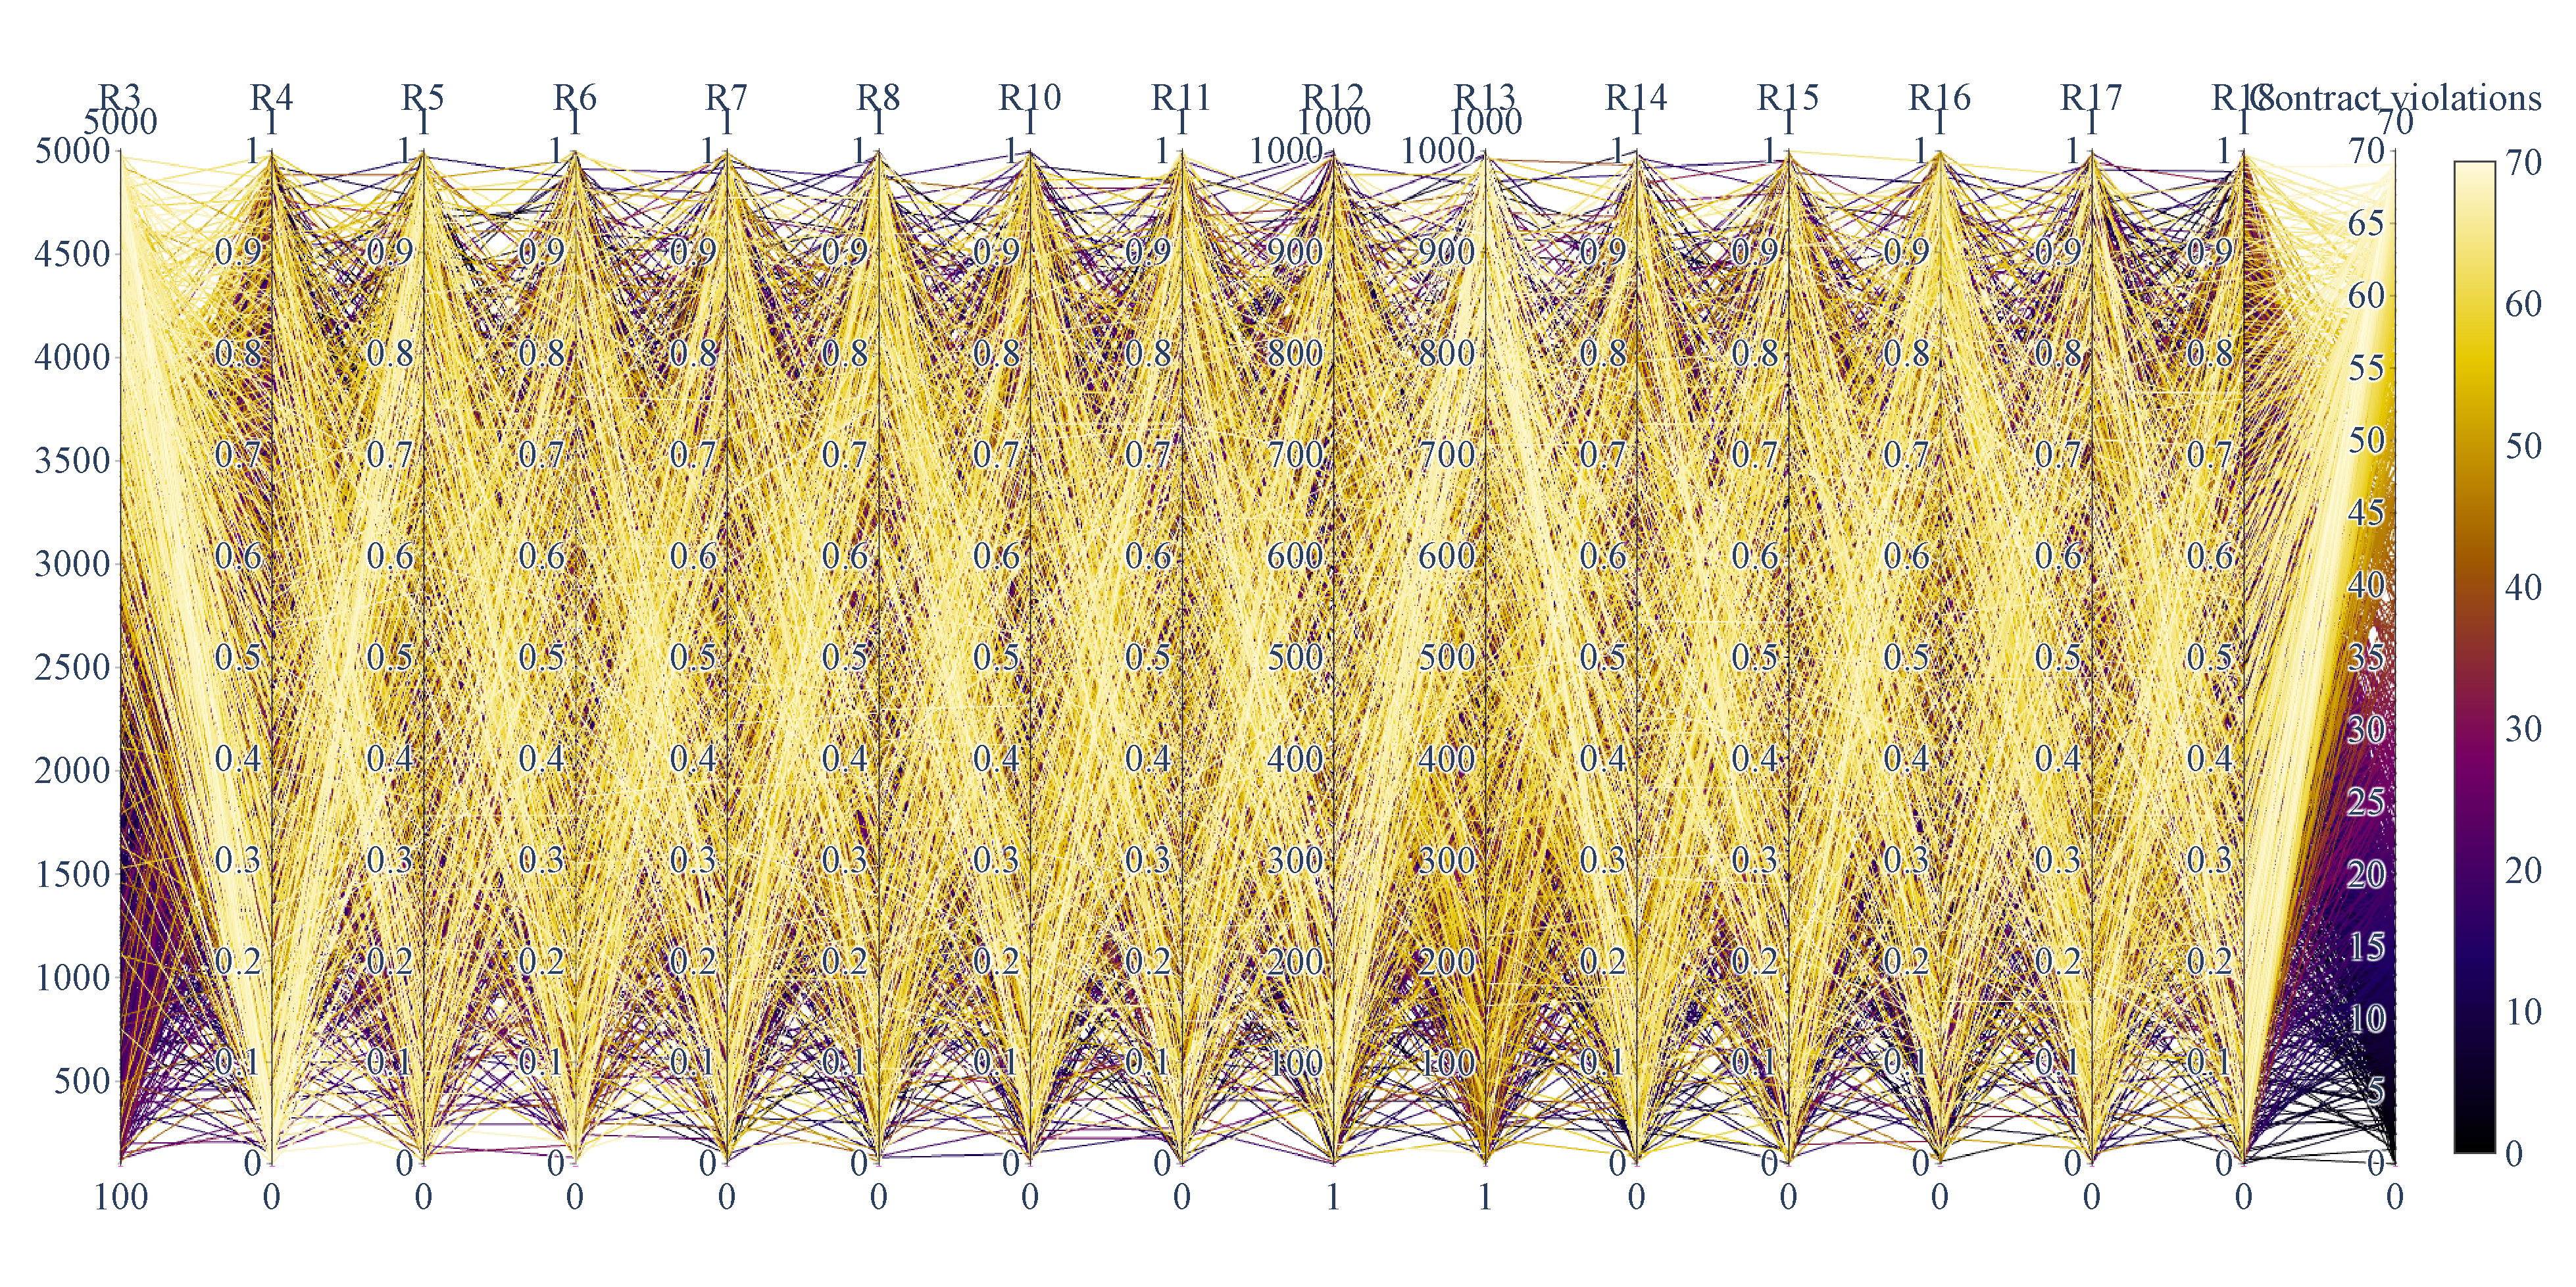
\includegraphics[width=\textwidth]{images/SPEA2.pdf}
	\caption[]]{}
	\label{fig:SearchSpaceViewFull}
\end{figure}

There is not much useful information. Among the configurations, there are those that led to valid results (the number of contract violations is 0) and many that led to more contract violations.

\begin{figure}
	\centering
	\includegraphics[width=\textwidth]{images/SPEA2_Zero_validity.html.pdf}
	\caption[]]{}
	\label{fig:SearchSpaceValid}
\end{figure}

Filtering out only those configurations that gave valid results, we got the search space shown in Figure~\ref{fig:SearchSpaceValid}. From the Figure~\ref{fig:SearchSpaceValid} it follows that there are no apparent dependencies between the parameters and the number of contract violations, or between the parameters themselves.

\begin{figure}
	\centering
	\includegraphics[width=\textwidth]{images/CorrelationAnalysis.pdf}
	\caption[]]{}
	\label{fig:CorrelationAnalysis}
\end{figure}

Cause Figure~\ref{fig:SearchSpaceViewFull} and Figure~\ref{fig:SearchSpaceValid} shows that search space view could not give any conclusions about dependencies between parameters or between parameters and number of contract violations, another method of analysis was performed.
We made a correlation analysis and it showed in Figure~\ref{fig:CorrelationAnalysis}. Colors indicate the level of correlation. Blue is the inverse correlation, that means that bigger value of parameter gives smaller number of contract violations. Red color means that bigger value o parameter gives bigger number of contract violations.
From the correlation analysis, we can conclude that there are no strong dependencies between the number of contract violations and parameters. There are two more important parameters: \texttt{CrossoverRate}(R5) and \texttt{CrossoverOnRandomRequestProbability}(R16).
Correlation analysis showed that the \texttt{CrossoverRate} need to has a big value. Also, conclusion from this analysis that small value  \texttt{CrossoverOnRandomRequestProbability}. It's also shows that we can remove this parameter. 

For further analysis of dependencies, graphs of the distribution of parameter pairs were constructed. Let us examine one representative distribution and, using another as an example, show how others look.

\begin{figure}
	\centering
	\includegraphics[width=\textwidth]{images/CrossoverRateVsutationRate.pdf}
	\caption[]]{}
	\label{fig:CrossoverRateVmutationRate}
\end{figure}

\begin{figure}
	\centering
	\includegraphics[width=\textwidth]{images/populatioSizeVsMu.pdf}
	\caption[]]{}
	\label{fig:populatioSizeVsMu}
\end{figure}

Any distribution associated with the population size parameter has a different look and shows that this parameter has an effect on the result.
Figure~\ref{fig:populatioSizeVsMu} shows an example of such distribution, and it is clearly seen that valid results, or close to valid, are in the range from 1000 to 2600.

At the same time, most distributions are similar to Figure~\ref{fig:CrossoverRateVsutationRate}, which shows the distribution of parameters of crossover rate and mutation rate. 
The Figure~\ref{fig:CrossoverRateVmutationRate} shows that valid, or close to valid results exist for all values of described parameters. That also confirms idea described in correlation analysis to remove some parameters like \texttt{CrossoverOnRandomRequestProbability} from the tuning and set it in the solver as 0.

\begin{figure}
	\subfloat[Name A]{%
		\includegraphics[clip,width=\textwidth]{images/populationSize_gradientBig.png}%
	}
	
	\subfloat[Name b]{%
		\includegraphics[clip,width=\textwidth]{images/populationSize_gradientSmall.png}%
	}
	
	\caption{main caption}	
\end{figure}

The next step in the analysis is the distribution of the parameter value and the number of contract violations that he gave. Consider the distribution of the population size parameter.
The color indicates the number of contract violations. The column height of a specific color is a percentage of the total number of configurations that have the same value. As can be seen, valid solutions are in the range from 1000 to 2600, which confirms the conclusion from the last step.

For a more visual image, we construct a similar graph for the smaller problem. This problem described with parameters: variants - 2, depth - 2, requests - 2, resources - 5.
It is shown in Figure~\ref{fig:populationSize_gradientSmall}. If we compare Figure~\ref{fig:populationSize_gradientSmall} and Figure~\ref{fig:populationSize_gradientBig}, we can see that they have a similar distribution.

\begin{figure}
	\centering
	\includegraphics[width=\textwidth]{images/mutationRate_gradient_500dpi.png}
	\caption[]]{}
	\label{fig:mutationRate_gradient}
\end{figure}

The distributions of most parameters look like the distribution of the mutation rate parameter outlined in Figure~\ref{fig:mutationRate_gradient}.

Such a distribution means that the result of the solver does not matter from the value of the specific parameter.

\begin{figure}
	\centering
	\includegraphics[width=\textwidth]{images/populationSizeObjective.pdf}
	\caption[]]{}
	\label{fig:populationSizeObjective}
\end{figure}

As for energy, let's build the distribution of the obtained energy values for the same parameters (Figure~\ref{fig:populationSizeObjective}).

This distribution proves the fact that if the solver found a valid solution, then this solution is optimal, or close to it.